\documentclass{article}
\usepackage[utf8]{inputenc}

\title{Laboppgave}
\date{\today}


\usepackage[backend=biber,style=ieee,sorting=none]{biblatex}
\usepackage{graphicx}
\usepackage{glossaries}
\usepackage{placeins}
\usepackage{listings}
\usepackage{todonotes}

\bibliography{references}

\lstset{
frame = single, 
language=Bash,
extendedchars=false,
columns=fullflexible, 
basicstyle=\ttfamily,
breaklines=true,
postbreak=\mbox{\textcolor{red}{$\hookrightarrow$}\space}
}

\begin{document}

\newacronym{ros}{ROS}{Robot Operating System}
\newacronym{ros-i}{ROS-I}{ROS Industrial}
\newacronym{urdf}{URDF}{Unified Robot Description Format}


\maketitle

\section{Introduksjon}
Denne oppgaven er ment å gi en introduksjon til \gls{ros}, samt bruk av \gls{ros} med industriroboter. 


\subsection{KUKA KR-16}
Dere skal bruke to KR-16 roboter fra KUKA. Disse robotene kan ha en nyttelast på 16 kg, og er markedsførst som fleksible roboter for bruk til oppgaver som sveising, lakkering, pakking og montering.

En av robotene er montert på en traverskran. Dette øker arbeidsområdet betraktelig, og gjør at man f.eks kan gripe rundt et objekt fra flere forskjellige vinkler uten å måtte flytte selve objektet.  

I likhet med robotene i "Den andre labboppgaven\todo{sett inn navn på ABB labben}" har robotene 6 ledd, hvor 3 av disse er samlet til en håndledd. Mer innformasjon om matematisk modellering og oppbygning av en robotarm finner dere i "Den andre labboppgaven\todo{sett inn navn på ABB labben}".


Kontrollskapene for robotene ble designet i 2005, og har ganske begrenset regnekraft. Vi ønsker derfor å bruke et ekstern system for å planlegge og kontrollere robotbevegelsene. I "Den andre labboppgaven\todo{sett inn navn på ABB labben}" vil dere får mulighet til å programmere direkte på kontrollskapet fra ABB, ved hjelp av en teach pendant\todo{Har vi et ord for teach pendant på norsk?}. I denne oppgaven vil dere bruke \gls{ros} for å styre robotene fra en ekstern PC som kjører Linux. 

\subsubsection{Tekniske data}

\begin{table}[!htbp]
\centering
%\resizebox{\textwidth}{!}{%
\begin{tabular}{l|l|l}
Axis & Range         & Speed   \\ \hline
A1   & $\pm$ 185$^{\circ}$        & 156$^{\circ}$/s \\
A2   & +35$^{\circ}$ /- 155$^{\circ}$  & 156$^{\circ}$/s \\
A3   & +154$^{\circ}$ /- 130$^{\circ}$ & 156$^{\circ}$/s \\
A4   & $\pm$ 350$^{\circ}$        & 330$^{\circ}$/s \\
A5   & $\pm$ 130$^{\circ}$        & 330$^{\circ}$/s \\
A6   & $\pm$ 350$^{\circ}$        & 615$^{\circ}$/s
\end{tabular}%
%}
\caption{Teknisk data KR-16\cite{kuka:kr16}}
\label{tab:kr16_range}
\end{table}


\begin{table}[!htbp]
\centering
%\resizebox{\textwidth}{!}{%
\begin{tabular}{l|l|l|l}
                          & \multicolumn{1}{l}{X-axis} & \multicolumn{1}{l}{Y-axis} & \multicolumn{1}{l}{Z-axis} \\ \hline
Max stroke                & 1500mm                     & 4800mm                     & 1500mm                     \\
Max velocity              & 0.5 m/s                    & 0.83m/s                    & 0.56m/s                    \\
Max acceleration          & 1 m/$s^2$                  & 1m/$s^2$                   & 1m/$s^2$                   \\
Calibration point offsets & 1517.5mm                   & 3700mm                     & -200mm                     \\
Repeatability             & \multicolumn{3}{c}{0.4mm}                                                           
\end{tabular}%
%}
\caption{Teknisk data traverskran\cite{SINTEF:robotlab}}
\label{tab:gantry}
\end{table}

\begin{figure}[!htbp]
    \centering
    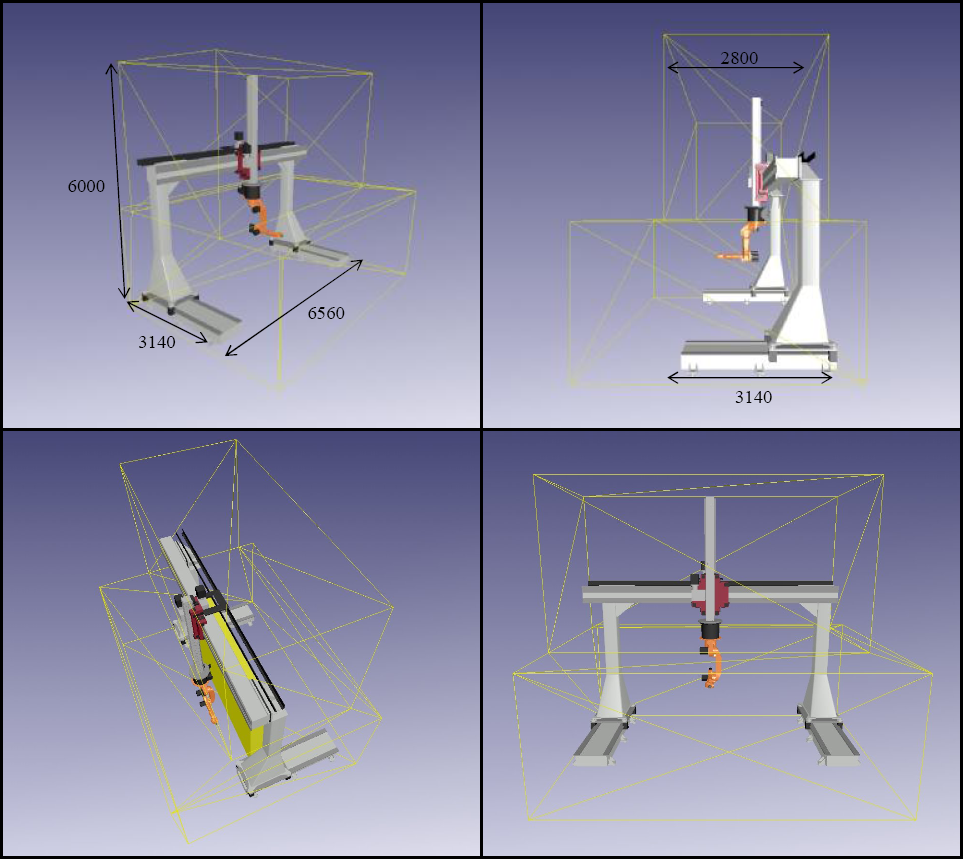
\includegraphics[width=\textwidth]{img/sintef_gantry}
    \caption{Dismensions for the gantry. Yellow lines marks available space\cite{SINTEF:robotlab}}
    \label{fig:gantry_envelope}
\end{figure}


\clearpage

\subsection{Robot Operating System}
\FloatBarrier

\gls{ros} er et åpen-kildekode rammeverk for roboter. Det startet som et prosjekt i robotikkmiljøet ved Stanford University, og ble videreutviklet av Willow Garage fra 2009 - 2013. Pr juli 2016 har \gls{ros} støtte for over 100 roboter, og er tatt i bruk over hele verden\cite{ros:metrics}. 


De mest brukte programmeringsspråkene i \gls{ros} er C++ og Python, men det er også støtte for LISP, Java og LUA.

\paragraph{Noder} i \gls{ros} er programmer som er laget for gjøre en spesifikk oppgave. Dette gjør at et system vanligvis består av flere noder, som samarbeider om å fullføre en kompleks oppgave. Figure \ref{fig:ros_topics} er et eksempel på et enkelt system for å lese leddvinkler fra en robot og lage en kinematisk modell av denne. Systemet består av flere noder, som er markert som elipser. \emph{kuka\_hardware\_interface} står for kommunikasjonen mellom \gls{ros} og en fysiske roboten. \textit{robot\_state\_publisher} regner ut alle transformasjonene som er nødvendig for å vise tilstanden til roboten. 

\paragraph{Kommunikasjon} mellom nodene skjer via spesialiserte meldinger over kommunikasjonskanaler kalt "topics". Disse bruker er satt opp slik at alle noder kan sende meldinger inn på en \textit{topic}, eller abonnere på å få meldinger som er sendt til en \textit{topic}. I figur \ref{fig:ros_topics} er hver \textit{topic} markert i en firkant, og pilene viser hvilken vei meldingene går. Piler som peker fra en \textit{node} til en \textit{topic} marker at noden sender meldinger, mens en pil andre veien marker at en \textit{node} lytter på en \textit{topic}.

\begin{figure}[!htbp]
    \centering
    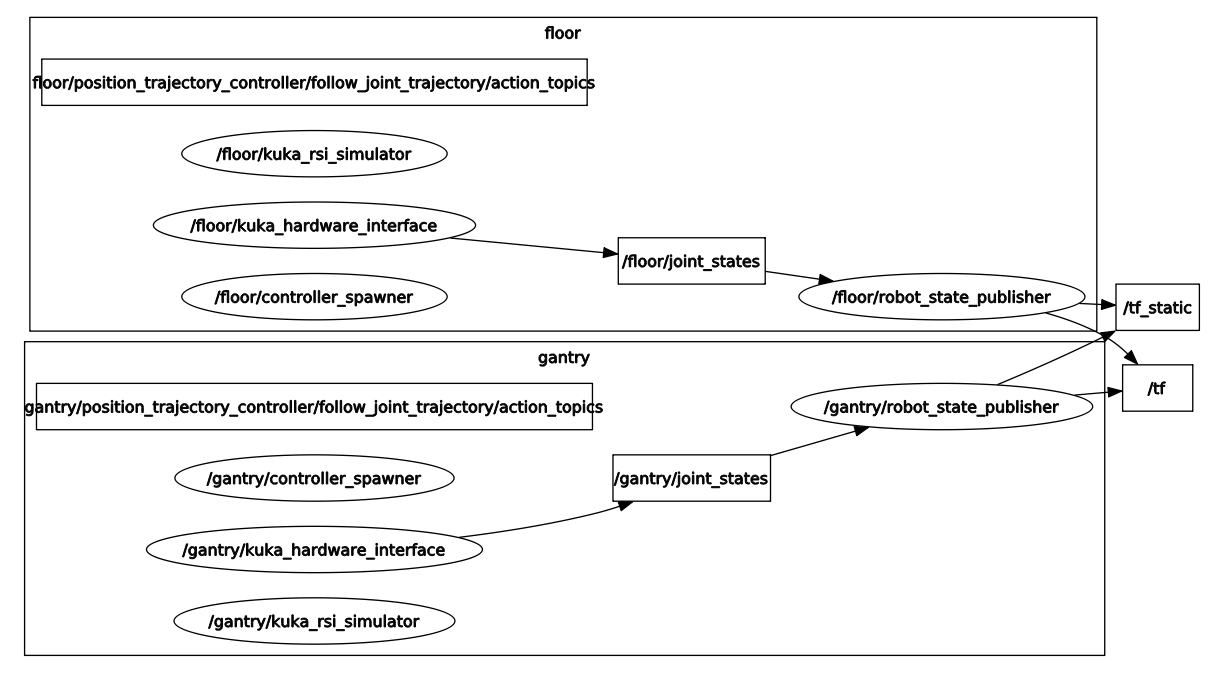
\includegraphics[angle=90,width=0.8\textwidth,height=0.8\textheight,keepaspectratio]{img/ros_topics}
    \caption{Example of nodes and topics in ROS}
    \label{fig:ros_topics}
\end{figure}


\paragraph{\gls{urdf}} er et XML format brukt for å beskrive roboter. Ved hjelp av elementer som lenker (links) og ledd (joints) kan man bygge komplekse modeller. En lenke kan være representert som en enkel geometrisk figur, eller bestå av mer komplekse 3D modeller. Dere kan finne \gls{urdf} fila som beskriver en KR-16 robot på \url{https://github.com/itk-thrivaldi/kuka_experimental/blob/master/kuka_kr16_support/urdf/kr16_2.urdf}  

\paragraph{Xacro} er et XML makro språk som gjør det lettere å jobbe med store \gls{urdf} modeller. I tilegg til en rekke innebygde funksjoner, har Xacro støtte for å inkludere andre filer. Dette gjør det enkelt å sette sammen komplekse modeller fra mindre filer. I denne labben skal dere blant annet bruke \url{https://github.com/itk-thrivaldi/thrivaldi_common/blob/master/robotlab_support/urdf/robotlab_macro.xacro}, som setter sammen flere mindre modeller til å bli robotene slik de står i labben.


\paragraph{rviz} er et visualiseringsverktøy for \gls{ros}, som dere skal bruke for å se en 3D modell av labben, og teste bevegelsene før dere kjører de på robotene.

\paragraph{MoveIt!} er et Scan'n'Plan rammeverk. Bruksområdet er typisk å scanne et arbeidsområde, detektere objekter for å så planlegge manipulering av objektene. Vi skal ikke bruke MoveIt! for å kontrollere robotene, men dere kan kjøre MoveIt! med en simulert versjon av labben om dere ønsker det. 


\clearpage
\section{Utførelse på laben}
Oppgaven delvis basert på \gls{ros} veiledningen\footnote{\url{http://wiki.ros.org/ROS/Tutorials}}, og dere vil kunne finne utdypende informasjon i den. Om dere ønsker så kan mesteparten av denne laboppgaven gjøres på en virtuell Ubuntu installasjon som dere kan kjøre på en egen PC. Innformasjon om oppsett og installasjon av denne finnes i \gls{ros-i} innføringen\footnote{\url{http://ros-industrial.github.io/industrial_training/_source/setup/PC-Setup---ROS-Kinetic.html}} 

Dere skal bruke en PC som kjører Linux (Ubuntu 16.04), og det meste dere skal gjøre kan og/eller må gjøres via en terminal. Denne finner dere i menyen på venstre side av skjermen. 
\subsubsection*{Noen nyttige kommandoer}
\begin{description}
\item[cd] (change directory) Flytter dere til en annen katalog
\item[ls] (list) Lister alle filer og kataloger
\item[pwd] (print work directory) Gir dere stien til den katalogen dere er i nå
\item[mkdir] (make directory) Lager en katalog
\item[rm] (remove) Sletter en fil eller katalog
\end{description}

\subsubsection*{Noen nyttige \gls{ros} spesifikke kommandoer}
\begin{description}
\item[roscd] Som \texttt{cd} men tar inn \gls{ros} pakkenavn som argument
\item[catkin\_make] Kompilerer \gls{ros} pakkene som er i et arbeidsområde
\item[roslaunch] Starter et \gls{ros} script
\end{description}

\subsection{Sett opp arbeidsområde}
For å holde orden på script og programmer som ikke er en del av den offisielle \gls{ros} distribusjon bruker vi Catkin.
Catkin samler disse i et arbeidsområde (workspace) som inneholder kildekode og har støttefunksjoner for å kompilere kildekoden  til kjørebare programmer. Vi skal først fjerne eventuelle rester etter forrige gruppe, før vi lager setter opp en nytt arbeidsområde som skal brukes i resten av labben. \\
 
 
\noindent\textbf{Last inn standard \gls{ros} variabler:}
\begin{lstlisting}[language=bash]
source /opt/ros/kinetic/setup.bash
\end{lstlisting}

\noindent\textbf{Slett arbeidsområdet til forrige gruppe hvis det finnes:}
\begin{lstlisting}[language=bash]
rm -rf ~/catkin_ws
\end{lstlisting}

\noindent\textbf{Lag en katalog til arbeidsområdet:}
\begin{lstlisting}[language=bash]
mkdir -p ~/catkin_ws/src
\end{lstlisting}

\noindent\textbf{Bytt katalog til arbeidsområdet:}
\begin{lstlisting}[language=bash]
cd ~/catkin_ws
\end{lstlisting}

\noindent\textbf{Lag nødvendig konfigurasjon for arbeidsområdet:}
\begin{lstlisting}[language=bash]
catkin_make
\end{lstlisting}

\noindent\textbf{Last variabler fra det nyopprettede arbeidsområdet:}
\begin{lstlisting}[language=bash]
source devel/setup.bash 
\end{lstlisting}

\subsection{Installer ROS pakker for robotlaben}
\label{install_support}
Vi må installere tre pakker for å kunne bruke \gls{ros} til å kontrollere robotene. To av disse inneholder modeller og \gls{urdf} filer som beskriver labben, mens den siste er driveren som vi bruker for å kommunisere med kontrollskapene fra KUKA. Alle pakkene ligger på GitHub\footnote{\url{https://github.com/itk-thrivaldi}}, som gjør at vi kan bruke git\todo{burde hatt med en beskrivelse av git} for å laste ned pakkene.\\


\noindent\textbf{Bytt katalog til kildekode katalogen i arbeidsområdet:}
\begin{lstlisting}[language=bash]
cd ~/catkin_ws/src/
\end{lstlisting}

\noindent\textbf{Last ned \texttt{kuka\_experimental} pakken fra GitHub:}
\begin{lstlisting}[language=bash]
git clone https://github.com/itk-thrivaldi/kuka_experimental
\end{lstlisting}

\noindent\textbf{Last ned \texttt{thrivaldi\_common} pakken fra GitHub:}
\begin{lstlisting}[language=bash]
git clone https://github.com/itk-thrivaldi/thrivaldi_common
\end{lstlisting}

\noindent\textbf{Last ned \texttt{kuka\_kvp\_hw\_interface} pakken fra GitHub:}
\begin{lstlisting}[language=bash]
git clone https://github.com/itk-thrivaldi/kuka_kvp_hw_interface
\end{lstlisting}

\noindent\textbf{Bytt katalog til arbeidsområdet:}
\begin{lstlisting}[language=bash]
cd ~/catkin_ws
\end{lstlisting}

\noindent\textbf{Installer evnetuelle manglende \gls{ros} pakker:}
\begin{lstlisting}[language=bash]
rosdep install --from-path src --ignore-src
\end{lstlisting}

\noindent\textbf{Kompiler all kildekode i arbeidsområdet:}
\begin{lstlisting}[language=bash]
catkin_make
\end{lstlisting}

\noindent\textbf{For å være sikker på at \gls{ros} finner pakkene vi har installert må vi laste inn system-variablene på nytt:}
\begin{lstlisting}[language=bash]
source ~/catkin_ws/devel/setup.bash 
\end{lstlisting}

\subsection{Lag ROS pakke}
\label{create_package}
For å kunne lage et eget program for å bevege robotene trenger vi først å lage en Catkin pakke. \\

\noindent\textbf{Bytt katalog til kildekode katalogen i arbeidsområdet:}
\begin{lstlisting}[language=bash]
cd ~/catkin_ws/src/
\end{lstlisting}

\noindent\textbf{Bruk Catkin for å opprette en ny pakke:}
\begin{lstlisting}[language=bash]
catkin_create_pkg ttk4100 rospy std_msgs 
\end{lstlisting}

For at \gls{ros} programmene skal finne pakken vår, må vi kompilere den og laste inn 
\noindent\textbf{Bytt katalog til arbeidsområdet:}
\begin{lstlisting}[language=bash]
cd ~/catkin_ws
\end{lstlisting}

\noindent\textbf{Kompiler all kildekode i arbeidsområdet:}
\begin{lstlisting}[language=bash]
catkin_make --pkg ttk4100
\end{lstlisting}

\noindent\textbf{For å være sikker på at \gls{ros} finner pakkene vi har opprettet må vi laste inn system-variablene på nytt:}
\begin{lstlisting}[language=bash]
source devel/setup.bash 
\end{lstlisting}

\noindent\textbf{Vi kan nå bruke roscd for å bytte katalog til pakken vår:}
\begin{lstlisting}[language=bash]
roscd ttk4100
\end{lstlisting}

Mer info om å lage \gls{ros} pakker finnes på \url{http://wiki.ros.org/ROS/Tutorials/CreatingPackage}

\subsection{Visualisering av labben}
For å sjekke at \gls{urdf} filene er korrekt installert, skal vi laste disse til en parametertjener, for å så visualisere modellen i rviz. Siden dette krever at flere \gls{ros} noder kjører samtidig, skal vi lage en \texttt{launch} fil som starter alle nodene for oss. Denne skal vi plassere i en underkatalog \texttt{launch} i pakken vår. \\


\noindent\textbf{Opprett launch katalogen:}
\begin{lstlisting}[language=bash]
mkdir launch
\end{lstlisting}
 
\noindent\textbf{Start et enkelt tekstbehandlingsprogram:}
\begin{lstlisting}[language=bash]
gedit launch/test.launch
\end{lstlisting}
 
 \noindent\textbf{Skriv eller kopier koden over til test.launch:}
\begin{lstlisting}[language=xml,numbers=left,stepnumber=1]
<?xml version="1.0"?>
<launch>
  <include file="$(find robotlab_support)/launch/load_robotlab.launch" />
  <node name="joint_state_publisher" pkg="joint_state_publisher" type="joint_state_publisher">
    <param name="use_gui" value="true" />
  </node>
  <node name="robot_state_publisher" pkg="robot_state_publisher" type="robot_state_publisher"/>
  <node name="rviz" pkg="rviz" type="rviz" args="-d $(find robotlab_support)/config/rviz.rviz" required="true" />
</launch>
\end{lstlisting}

Linje 3 laster \gls{urdf} beskrivelsen av robotene til paramtertjeneren. Linje 4 og 7 starter støtteprogrammer som generer informasjonen om leddvinkler. Med en virkelig robot ville denne innformasjonen vært hentet fra roboten. Linje 8 starter rviz, som vi bruker for å gi en grafisk representasjon av robotene.

\noindent\textbf{Etter å ha lagret fila, og lukket gedit kan vi kjøre den:}
\begin{lstlisting}[language=bash]
roslaunch ttk4100 test.launch
\end{lstlisting}

Hvis alt fungerer som det skal ser dere nå en grafisk representasjon av robotene, og en boks hvor dere kan sette verdien på leddene til robotene. Når dere forander på disse skal modellen oppdatere seg fortløpende.

Når dere er klar for å gå videre, kan dere trykke \textbf{ctrl+c} i terminalvinduet. Dette avslutter den kjørende prossesen.

\subsection{Last ned filer}
I tilegg til de tre pakkene som ble lastet ned fra GitHub i steg \ref{install_support} er det gjort klar noen filer som skal brukes i pakken dere opprettet i steg \ref{create_package}. Denne inneholder koden som vi skal bruke for å bevege roboten, og inneholder kommentarer som forklarer hva vert steg gjør.

\noindent\textbf{Last ned filer\todo{Her må dere finne ut hva som er beste måten å distribuere filene på}:}
\begin{lstlisting}[language=bash]
wget https://github.com/ivareri/ttk4100/archive/master.zip
\end{lstlisting}

\noindent\textbf{Pakk ut de nedlastede filene\todo{Dette steget må tilpasses slik at de ender opp med script/ katalogen under roten på ttk4100 pakken}:}
\begin{lstlisting}[language=bash]
unzip master.zip
\end{lstlisting}

Dere har nå fått en ny katalog, \texttt{script} som inneholder filene vi skal bruke for å snu esken. 

\begin{description}
\item[floor.py] Inneholder navn på alle ledd, og forhåndsdefinerte posisjoner
\item[gantry.py] Samme som floor.py, men for Gantry roboten
\item[\_\_init\_\_.py] En tom fil. Den er nødvdening for at Python skal kunne importere andre filer fra katalogen
\item[RobotActionClient.py] Inneholder koden som sender posisjonene til \gls{ros}
\item[node.py] Den filen som dere skal kjøre. Den bruker RobotActionClient til å flytte robotene.
\end{description}

\noindent\textbf{Sett rett flag på \texttt{node.py} slik at den er kjørbar:}
\begin{lstlisting}[language=bash]
chmod +x scripts/node.py
\end{lstlisting}


\subsection{Simuler programmet}
I dette delen trenger dere to terminaler for å kunne simulere labben samtidig som dere kjører programmet.

\noindent\textbf{I terminal 1}
\begin{lstlisting}[language=bash]
roslaunch robotlab_support robot_state_visualize_robotlab.launch
\end{lstlisting}

\noindent\textbf{I terminal 2}
\begin{lstlisting}[language=bash]
rosrun ttk4100 node.py
\end{lstlisting}

Hvis alt fungerer skal dere ha fått opp et rviz vindu med robotlabben. Når dere starter \textt{node.py} skal robotene gå igjennom de samme beveglsene som vi ønsker å ha i labben. For å gjøre koden så enkel som mulig gjør vi ikke noe kollisjonsjekking. I det første steget vil robotene kollidere, men oppstartposisjonen i labben skal sørge for at det ikke skjer når dere kjører koden i lab.

Når programmet har kjørt ferdig, og studassen er fornøyd med bevegelsene kan dere lukke rviz og gå videre til å kjøre koden på robotene.

\subsection{Kjør programmet på roboten}
Vi må lage en ny launch fil for å starte robotdriveren og rviz. Denne skal være lik den forige dere lagde, bortsett fra at dere skal bytte ut \texttt{joint\_state\_publisher} seksjonen med robotdriveren. Det som skal ut er i den første kodeblokken, og det som skal inn er i den andre.


\begin{lstlisting}[language=xml]
<node name="joint_state_publisher" pkg="joint_state_publisher" type="joint_state_publisher">
  <param name="use_gui" value="true" />
</node>

\end{lstlisting}

\begin{lstlisting}[language=xml]
<include file="$(find robotlab_support)/launch/robot_interface_streaming_robotlab.launch" >
  <arg name="kvp_floor" value="true" />
  <arg name="kvp_gantry" value="true"/>
</include>
\end{lstlisting}


\noindent\textbf{I terminal 1, bytt ut robot.launch med navnet på filen dere lagde over}
\begin{lstlisting}[language=bash]
roslaunch ttk4100 robot.launch
\end{lstlisting}

\noindent\textbf{I terminal 2}
\begin{lstlisting}[language=bash]
rosrun ttk4100 node.py
\end{lstlisting}

\clearpage

\printbibliography
\end{document}
